\section{Hardware}
\label{sec:hardware}
Written in Arduino. \cite{ArduinoLanguageReference}

% \begin{figure}[h]
%     \centering
%     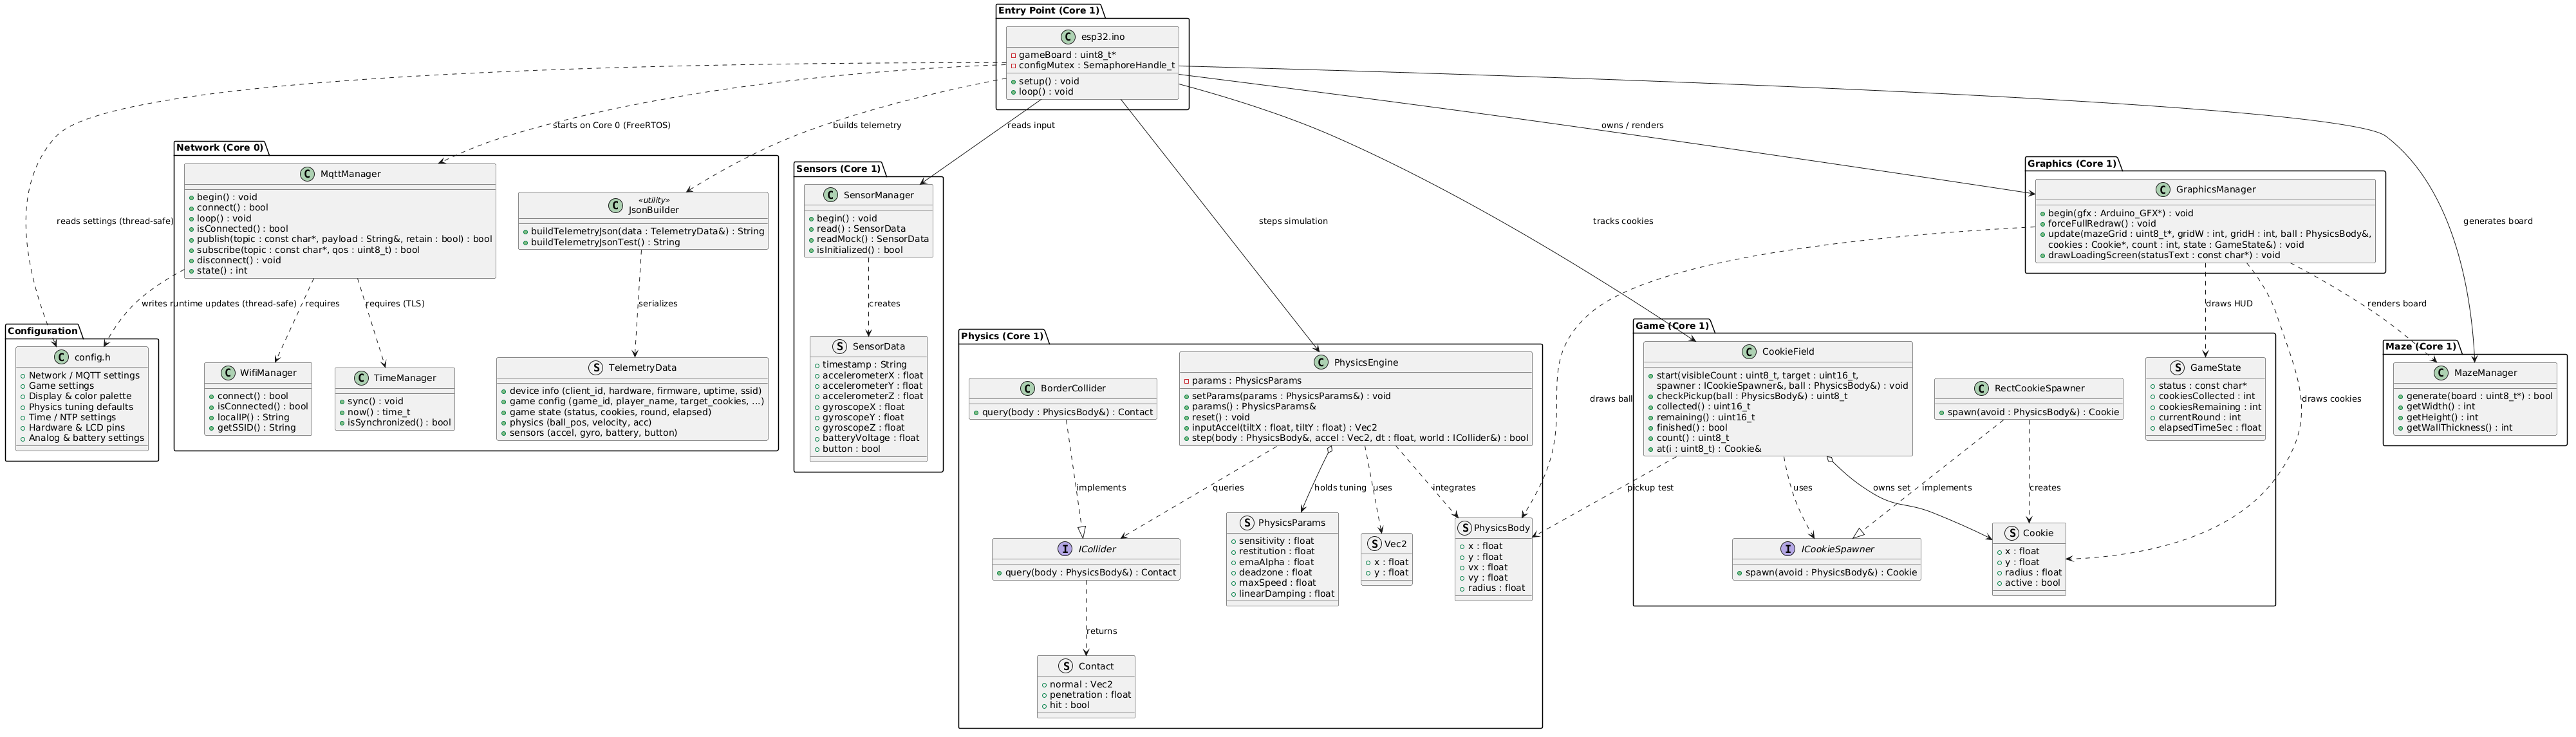
\includegraphics[width=0.9\linewidth]{../diagrams/out/architecture/architecture.png}
%     \caption[BiteBound Architecture]{System architecture diagram displaying modular firmware packages, cross-core memory boundaries, and execution contexts.}
%     \label{fig:architecture}
% \end{figure}

% sideways figure for better readability
\begin{sidewaysfigure}[p]
    \centering
    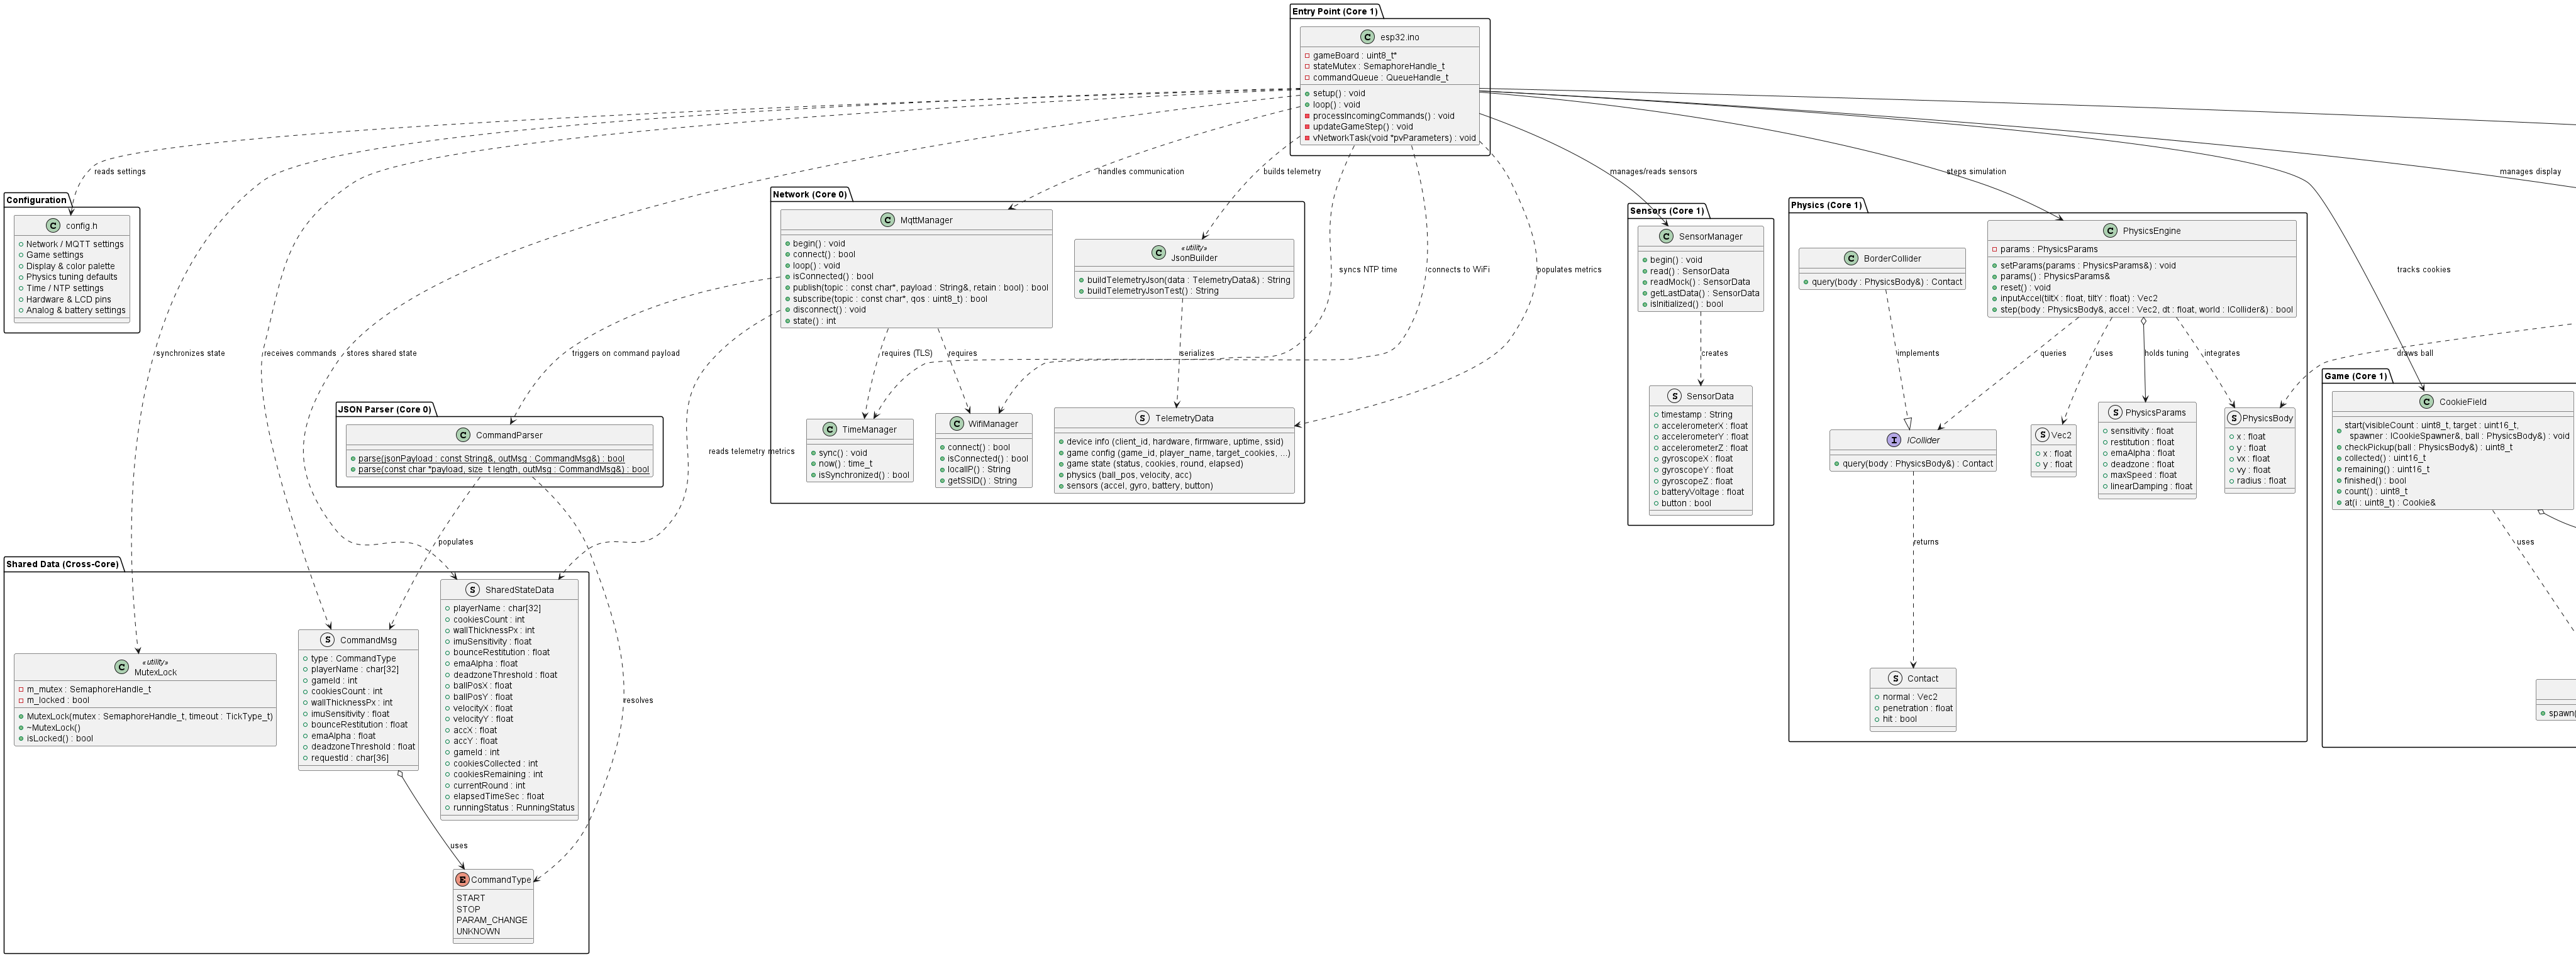
\includegraphics[width=\textheight]{../diagrams/out/hardware-architecture/hardware-architecture.png}
    \caption[BiteBound Hardware Architecture]{Hardware architecture UML diagram..}
    \label{fig:hardware-architecture}
\end{sidewaysfigure}

\subsection{ESP32-S3 Microcontroller}
\label{subsec:esp32_s3_microcontroller}
% TODO: write ESP32-S3 Microcontroller
% Describe the hardware components in detail, especially the ESP32-S3.
ESP32-S3: \cite{wavesharedoku}

\subsection{Concurrency}

\subsection{Sensor Data Acquisition}
\label{subsec:sensor_data_acquisition}
% TODO: write Sensor Data Acquisition
% Detail the data acquisition from the sensors and filtering.

\subsection{Physics Simulation \& Game Logic}
\label{subsec:physics_simulation_game_logic}
% TODO: write Physics Simulation & Game Logic
% Explain the physics simulation with its mathematical formulas.
% EMA usage for default_ema_alpha: \cite{klinker2011exponential}
% Bounce restitution: \cite{wang2017bounce}

\subsection{Display}
\label{subsec:display}
% TODO: write Display
% Detail the display logic and game mechanics with screenshots.

\subsection{MQTT Communication}
\label{subsec:mqtt_communication}
% TODO: write MQTT Communication
% Describe the MQTT communication setup, topics, and payloads.
